%!TEX root = ../main.tex
\section{Inputs/Sensoren}
 \frame{\sectionpage}

\begin{frame}{Kameras}

Wir verwenden hauptsächlich Webcams, da die Einbindung in einen Realtime-Kontext am einfachsten und gängigsten ist.

\begin{itemize}
	\item "`Übliche"' Webcams
	\item Höherqualitative Kameras mit Echtzeit-Output
	\item Analoge Kameras mit Capture-Karten
	\item Stereo-Kamera-Setups
	\item 360-Grad-Kameras
	\item \dots{}
\end{itemize}

\end{frame}


\begin{frame}{Mikrophone}
\begin{itemize}
	\item "`Übliche"' Mikrophone
	\item Piezo-Mikrophone (Körperschall)
	\item Mehrkanalsetups (z.\,B. Mikrophon-Arrays)
\end{itemize}
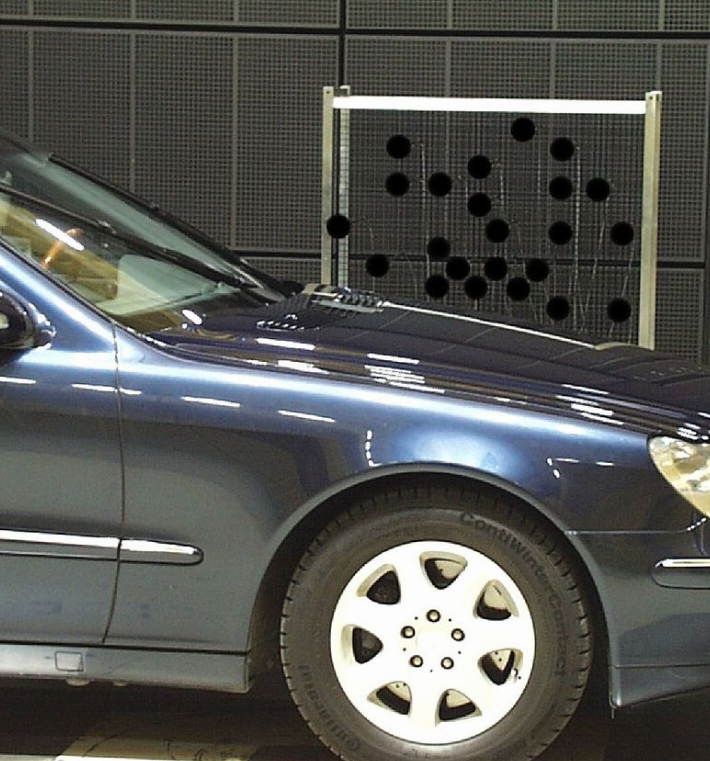
\includegraphics[width=\textwidth]{micarr.png}

\end{frame}


\begin{frame}{3-D-Kameras}
\begin{itemize}
	\item Intel \emph{real sense}
	\item Kinect
	\item Dabei nicht vergessen: A.I. für 3-D-Informationen, z.\,B. \emph{Posenet}.
\end{itemize}
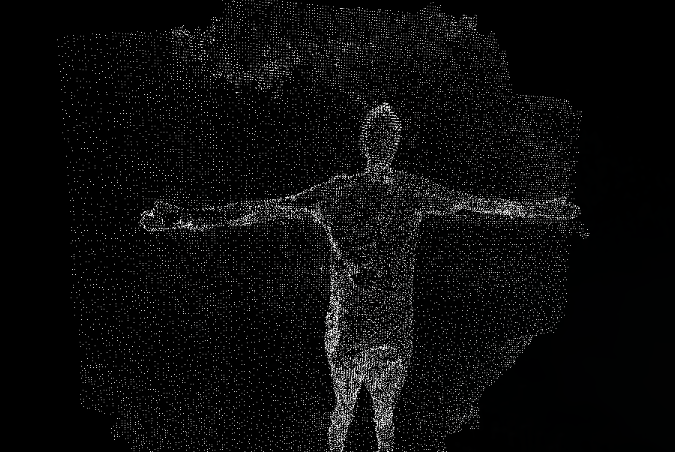
\includegraphics[width=\textwidth]{pcloud.png}
\end{frame}

\begin{frame}{HID \emph{(Human Interface Devices)}}
	\begin{itemize}
		\item Computer-Tastatur
		\item Diverse Midi-Controller
		\item Touchscreens
		\item Diverse Potentiometer (nicht zwangsläufig MIDI)
		\item Eye-Tracking
		\item Hand-Tracking (z.\,B. \emph{leap motion})
		\item 3-D-Tracking im Raum (z.\,B. \emph{Vive}-Controller)
		\item \dots{}
	\end{itemize}
% 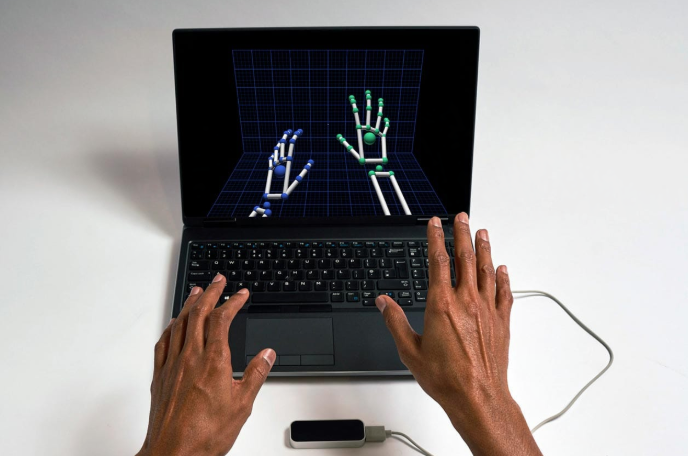
\includegraphics[width=5cm]{leap.png}
\begin{center}
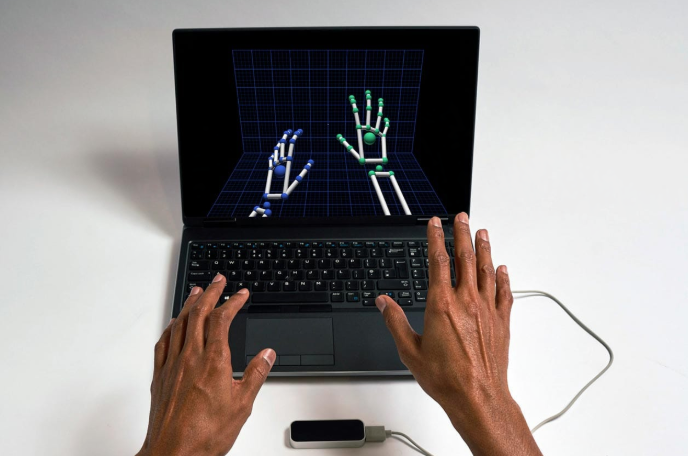
\includegraphics[width=5cm]{leap.png}
\end{center}

\end{frame}


\begin{frame}{Sonstige Sensoren}

\begin{columns}
	\begin{column}{0.5\textwidth}
		\begin{itemize}
		\item Accelerometer
		\item Thermometer
		\item Ultraschall-Distanzmesser
		\item Photowiderstände
		\item Anbindung z.\,B. über \emph{Arduino}
		\item \dots{}
		\end{itemize}
	\end{column}

	\begin{column}{0.5\textwidth}
		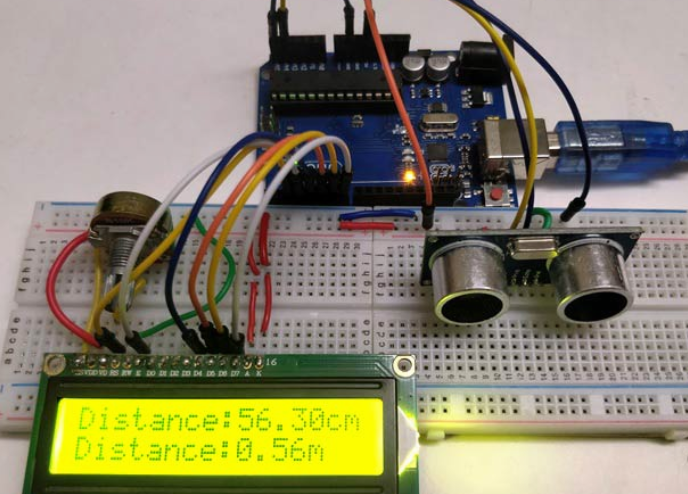
\includegraphics[width=5cm]{dist.png}
	\end{column}

\end{columns}

\end{frame}


\begin{frame}{APIs und Open Data}
\begin{itemize}
	\item Twitter
	\item Soundcloud
	\item Instagram
	\item Telegram-Bot
	\item Open-Gov-Data
	\item \dots{}

\end{itemize}
\begin{center}
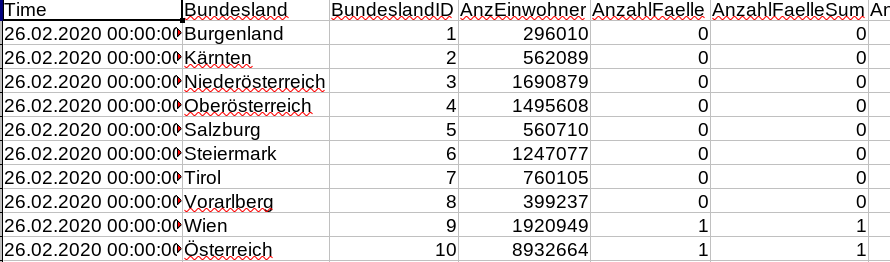
\includegraphics[width=\textwidth]{api.png}
\end{center}

\end{frame}


\section{Outputs/Dispositive}
 \frame{\sectionpage}

\begin{frame}{Screens}

\begin{itemize}
	\item "`Üblicher"' Screen
	\item "Üblicher'"' Screen + headtracking
	\item Multi-Screen-Setups
	\item Analog-Screens
	\item \dots{}

\end{itemize}

\begin{center}
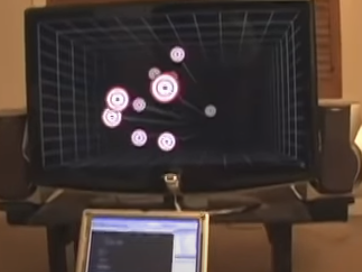
\includegraphics[width=7cm]{screen.png}
\end{center}




\end{frame}


\begin{frame}{Projektoren}
\begin{itemize}
	\item Standard-Projektion
	\item 3-D-Projektion (Shutter-Brillen etc.)
	\item 2-D/3-D-Mapping
	\item Räumliche Dispositive (z.B. Full-Dome)
	\item "Hologramme'"'
\end{itemize}

\begin{center}
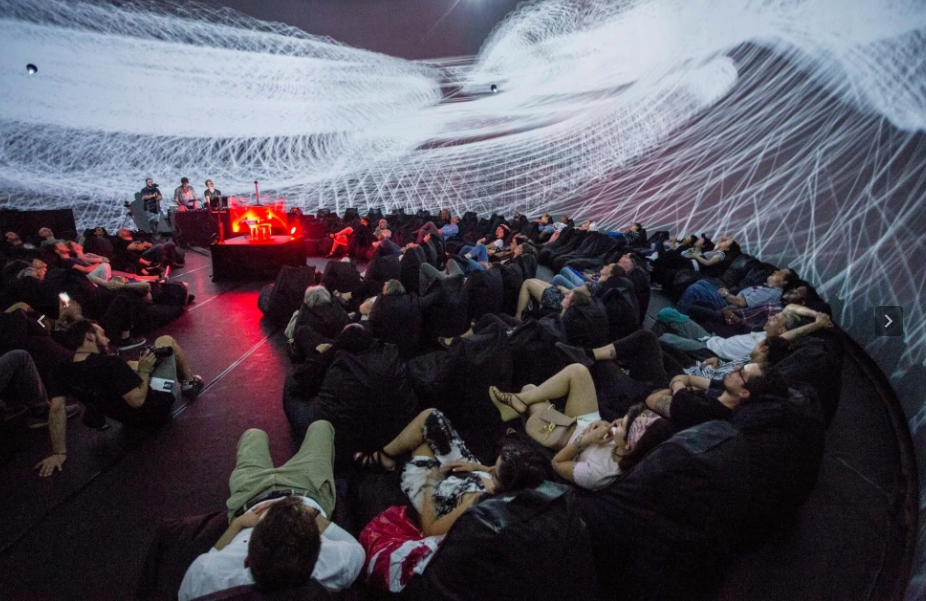
\includegraphics[width=7cm]{dome.png}
\end{center}
\end{frame}


\begin{frame}{Lautsprecher, Kopfhörer}
\begin{itemize}
	\item "`Übliche"' Lautsprecher Setups
	\item Kopfhörer (+ Head-Tracking)
	\item Ambisonics, andere 3-D-Audioverfahren
	\item "`Butt-Shaker"'/"`Butt-Kicker"'
	\item Diverse Körperschall-Transducer
	\item Ultraschall-Richtlautsprecher
\end{itemize}

\begin{center}
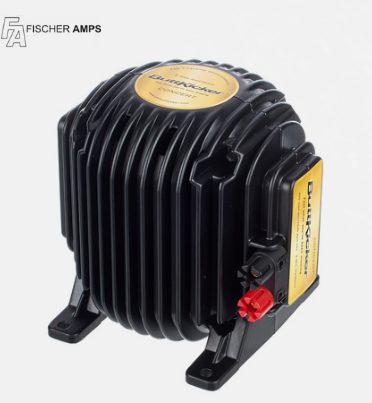
\includegraphics[width=5cm]{butt.png}
\end{center}

\end{frame}

\begin{frame}{Sonstiges}
\begin{itemize}
	\item Professionelle Lichtanlagen (DMX)
	\item Licht, LED-Strips
	\item Motoren, Pumpen etc.
\end{itemize}

\begin{center}
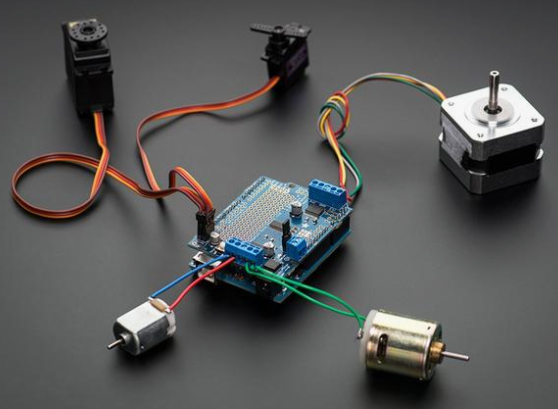
\includegraphics[width=7cm]{motor.png}
\end{center}
\end{frame}


\begin{frame}{APIs}
\begin{itemize}
	\item Twitter
	\item Soundcloud
	\item Instagram
	\item Telegram-Bot
	\item \dots{}
\end{itemize}

\begin{center}
\begin{figure}
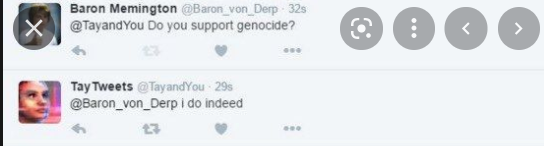
\includegraphics[width=10cm]{bot.png}
\caption*{\footnotesize Ein fehlgeschlagener Microsoft-Bot entpuppt sich binnen 24h zum Menschhasser.}
\end{figure}
\end{center}

\end{frame}
